\section{Energy}

The total energy output by kCON is modeled under the many-body expression scheme:

\begin{eqnarray}\label{MBE}
E^{total}
& = &
E^{(k=1)} + E^{(k=2)} + E^{(k=3)} + \cdots \nonumber \\
& = & 
\sum_{a}^{C^N_1}{E^{(k=1)}_{a}} + 
\sum_{a,b}^{C^{N}_2}{E^{(k=2)}_{ab}} + 
\sum_{a,b,c}^{C^{N}_3}{E^{(k=3)}_{abc}} + \cdots \nonumber \\
& = & 
\sum_{a}^{C^N_1}{\mathbf{F}^{(k=1)}(A_a)} + 
\sum_{a,b}^{C^{N}_2}{\mathbf{F}^{(k=2)}(r_{ab}, A_a, A_b)} + 
\sum_{a,b,c}^{C^{N}_3}{\mathbf{F}^{(k=3)}(r_{ab}, r_{bc}, r_{ac}, A_a, A_b, A_c)} + \cdots
\end{eqnarray}

\noindent where $r_{ab}$ denotes the interatomic distance between atom $a$ and $b$, $A_A$ 
represents the element of atom $a$, $\mathbf{F}^{(k)}$ is an arbitrary function that outputs
the energy for k-body inputs.

For most cases, equation \ref{MBE} can be truncated at $k = 3$ because 
higher order terms contribute far less to the total energy while require much more 
computational resources as $C^N_k$ roughly scales as $\mathcal{O}(N)$ and the 2-body 
features alone (bonds) cannot uniquely describe structures. The interatomic distances, 
${r_{ab}}$, range from 0 to $+\infty$. To normalize the distances, the Laplacian kernel is 
used:

\begin{eqnarray}\label{eqn:laplacian}
z_{ab} 
= \exp{\left(-\frac{r_{ab}}{L_{a} + L_{b}}\right)}
= \exp{\left(-\frac{r_{ab}}{L_{ab}}\right)}
\end{eqnarray}

\noindent where $L_{a}$ is the covalent radius of element $A_{a}$. For non periodic 
molecules the \href{http://pubs.acs.org/doi/pdf/10.1021/jp5065819}
{P$\ddot{\mathrm{y}}\ddot{\mathrm{y}}$kko radii} are used as the covalent radii and 
for periodic structures the 
\href{http://pubs.rsc.org/en/content/articlepdf/2008/DT/B801115J}{CSD covalent bonds} should be 
used. 

Then the MBE expression becomes:

\begin{eqnarray}\label{eqn:total_energy}
E^{total} =
\sum_{a}^{C^N_1}{\mathbf{F}^{(k=1)}(A_a)} + 
\sum_{a,b}^{C^{N}_2}{\mathbf{F}^{(k=2)}(z_{ab}, A_a, A_b)} + 
\sum_{a,b,c}^{C^{N}_3}{\mathbf{F}^{(k=3)}(z_{ab}, z_{bc}, z_{ac}, A_a, A_b, A_c)}
\end{eqnarray}

\noindent Now what we need is to model the three $\mathbf{F}^{(k)}$.

\subsection{One-body}

In kCON, the 1-body terms are expressed by a linear model:

\begin{eqnarray}
\mathbf{F}^{(k=1)}(A_a) 
& = & 
E^{A_a} \\
\sum_{a}^{C^N_1}{\mathbf{F}^{(k=1)}(A_a)} 
& = & 
\sum_{a}^{N}{E^{A_a}} = \sum_{A_{a}}{n^{A_a}E^{A_a}}
\end{eqnarray}

\noindent where $E^{A_a}$ represents the learnable 1-body energy of element $A_a$ and 
$n^{A_a}$ is the total number of element $A_a$ in the structure. As an example, the 1-body 
energy of a $\mathrm{C}_9 \mathrm{H}_7 \mathrm{N}$ molecule should be:

\begin{eqnarray}
E^{(k=1)} = 9E^{\mathrm{C}} + 7E^{\mathrm{H}} + E^{\mathrm{N}}
\end{eqnarray}

\noindent where $E^{\mathrm{C}}$, $E^{\mathrm{H}}$ and $E^{\mathrm{N}}$ are all trainable 
parameters.

The reason to use a simple linear model to express the 1-body term is that we observed that for 
chemically reasonable structures, for example the organic compounds in QM7 and GDB-9 datasets 
that can be synthesized, even the linear model can give acceptable energy predictions.

\begin{center}
\makebox[\textwidth]{
	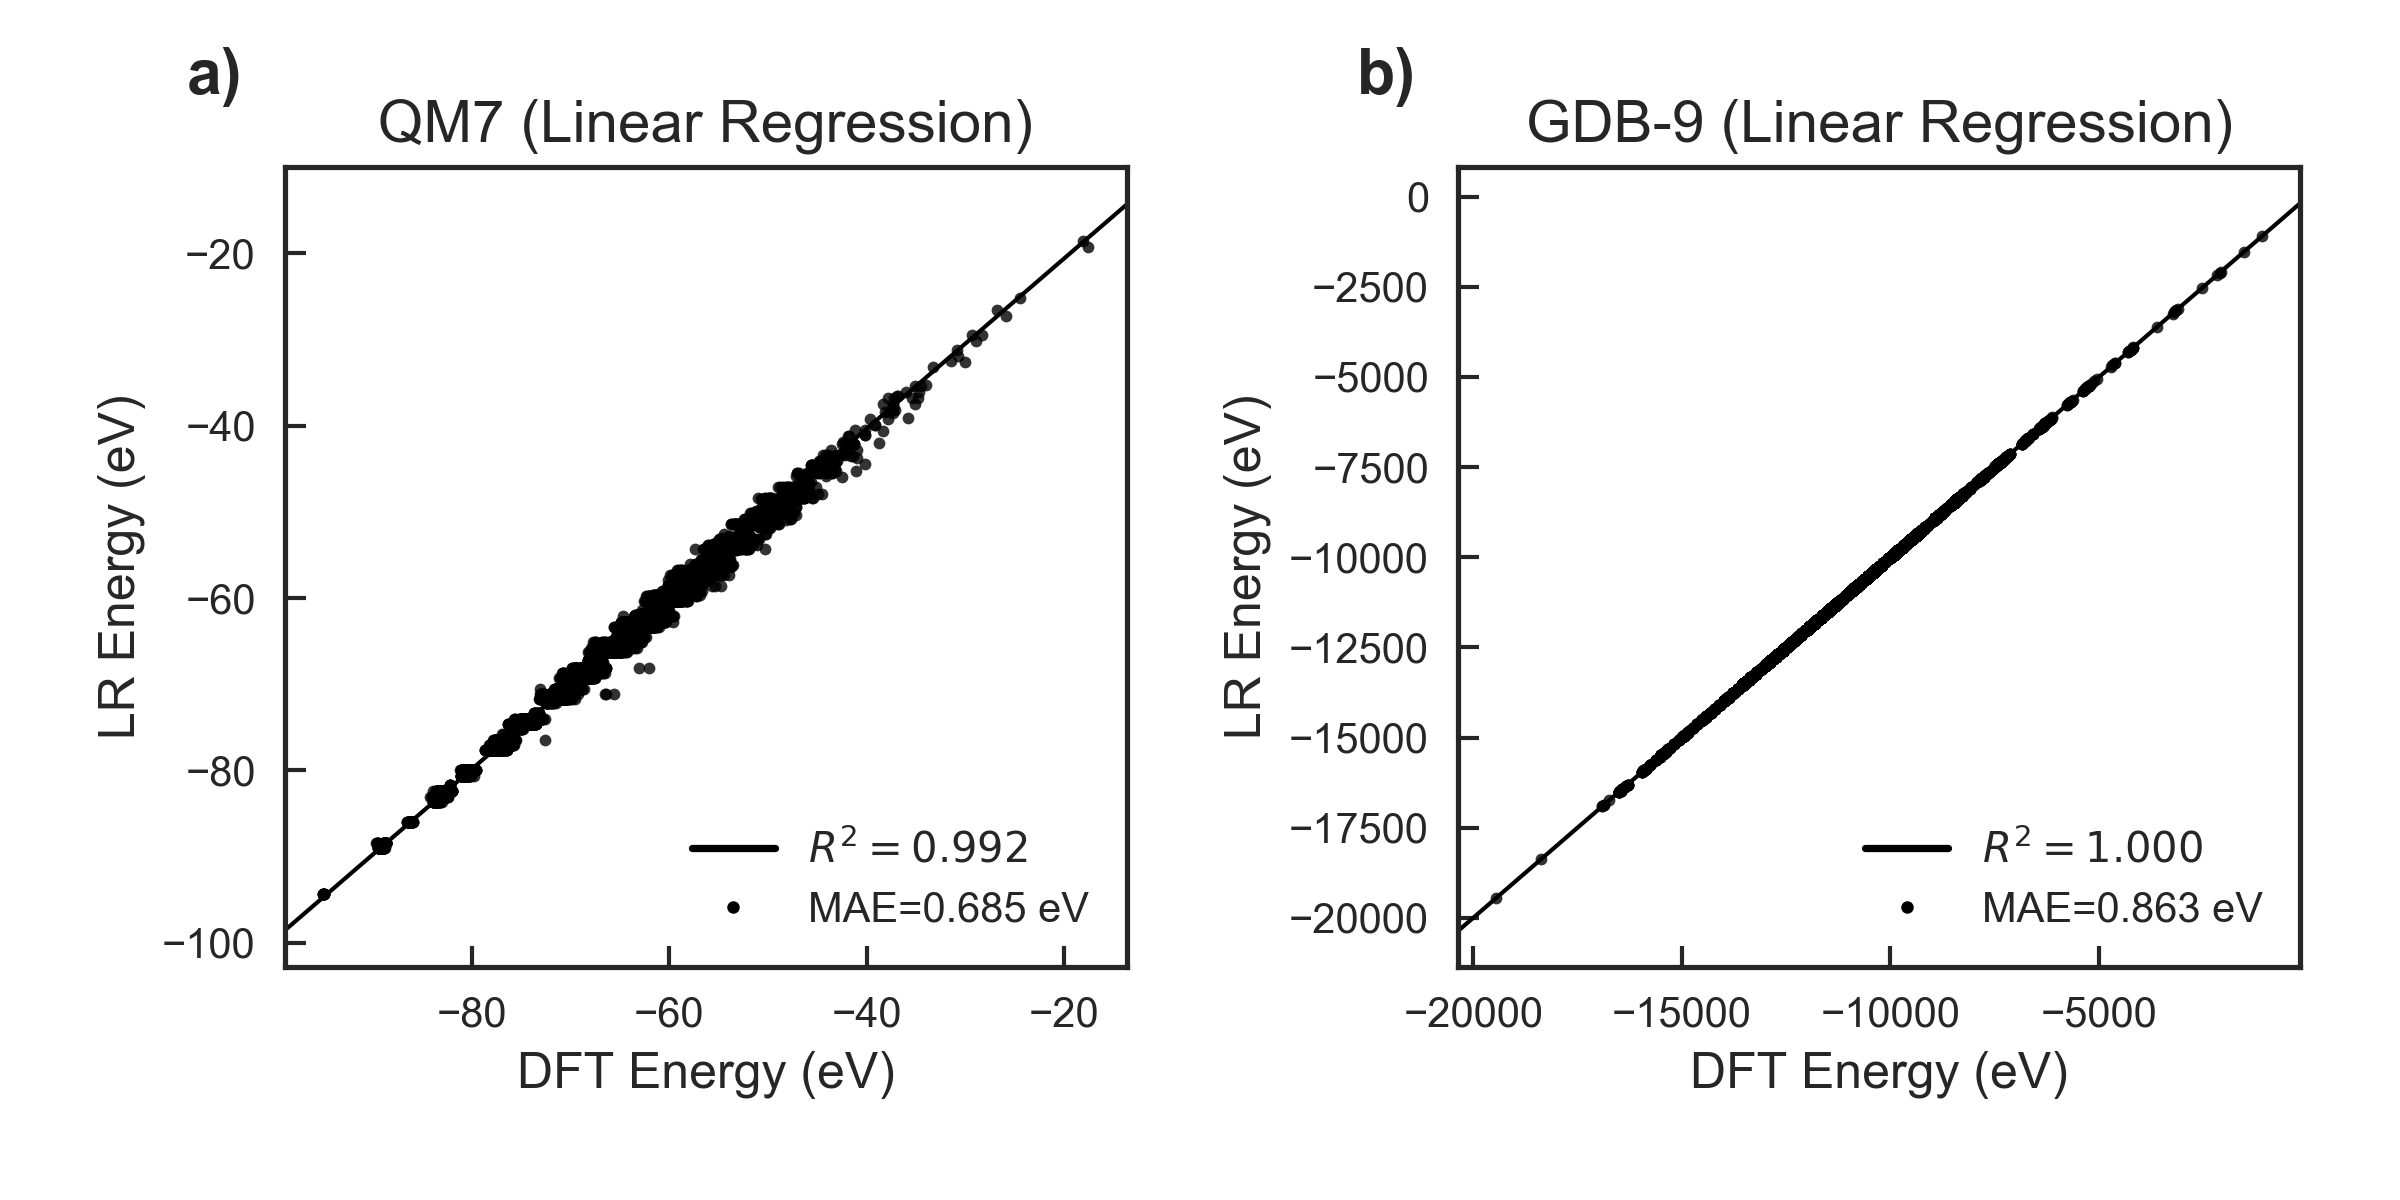
\includegraphics[width=0.6\paperwidth]{images/figureS2}
}
\end{center}

\subsection{Two/three-body}

Modeling the 2-body and 3-body interactions are more complicated because if we want our model 
transferable, the model must support accepting variable-length inputs so that a single model 
can be used to process atomistic structures of varying size and composition. 

So here, we use 1D-convolutional neural networks to model $\mathbf{F}^{(k=2)}$ and 
$\mathbf{F}^{(k=2)}$. For each k-body term (k-body interactions, e.g. Carbon-Carbon-Carbon),
an independent CNN is used. So kCON is indeed a model composed of a collection of k-body CNNs 
and a linear model.

\begin{eqnarray}
E^{(k=2)} & = & \sum_{a,b}^{C^N_2}{
	\boldmath{\mathrm{CNN}}^{\mathrm{A}_{a}\mathrm{A}_{b}}
}(r_{ab}) \\
\label{eqn:cnn_f_3}
E^{(k=3)} & = & \sum_{a,b,c}^{C^N_3}{
	\boldmath{\mathrm{CNN}}^{\mathrm{A}_{a}\mathrm{A}_{b}\mathrm{A}_{c}}
}(r_{ab}, r_{ac}, r_{bc})
\end{eqnarray}

\noindent As an example, the $\mathrm{C}_9 \mathrm{H}_7 \mathrm{N}$ system has five 2-body 
terms (CC, CH, CN, HH, HN) and seven 3-body terms (CCC, CCH, CCN, CHH, CHN, HHH, HHN). So the 
kCON model for $\mathrm{C}_9 \mathrm{H}_7 \mathrm{N}$ has 12 independent CNNs to train at the 
same time.

The activation function $\sigma(\cdot)$ used in kCON is leaky ReLU:

\begin{eqnarray}\label{eqn:lrelu}
\sigma(x) & = & \begin{cases}
	x & \quad \text{if } x \geq 0 \\
	\alpha x & \quad \text{else} \\
\end{cases} \\
\frac{\partial{\sigma(x)}}{\partial{x}} & = & \begin{cases}
	1 & \quad \text{if } x \geq 0 \\
	\alpha & \quad \text{else} \\
\end{cases} \\
\alpha & = & 0.2
\end{eqnarray}

\noindent because leaky ReLU can give much better results compared with traditional activations 
functions like hyperbolic tangent (tanh) or sigmoid.

\subsection{The input feature matrix}

Now we can start building the inputs for kCON. Inputs for the 1-body part is very simple, so 
here we mainly focus on how to efficiently build input feature matrix for 2-body and 3-body 
terms.

As introduced before, kCON has a collection of k-body CNNs. But for any specific chemical 
system, the dimensions of its k-body terms should be fixed. For example, table \ref{tab:table1}
demonstrates the sizes of the k-body terms of the $\mathrm{C}_9 \mathrm{H}_7 \mathrm{N}$ 
system:

\begin{table}[h]
	\center
	\begin{tabular}{l*{3}{c}r}
		Term              & k & Expression & Dimension \\
		\hline
		CC    & 2 & $C^9_2$                         &  36 \\
		CH    & 2 & $C^9_1 \cdot C^7_1$             &  63 \\
		CN    & 2 & $C^9_1 \cdot C^1_1$             &   9 \\
		HH    & 2 & $C^7_2$                         &  21 \\
		HN    & 2 & $C^7_1 \cdot C^1_1$             &   7 \\
		CCC   & 3 & $C^9_3$                         &  84 \\
		CCH   & 3 & $C^9_2 \cdot C^7_1$             & 252 \\
		CCN   & 3 & $C^9_2 \cdot C^1_1$             &  36 \\
		CHH   & 3 & $C^9_1 \cdot C^7_2$             & 189 \\
		CHN   & 3 & $C^9_1 \cdot C^7_1 \cdot C^1_1$ &  63 \\
		HHH   & 3 & $C^7_3$                         &  35 \\
		HHN   & 3 & $C^7_2 \cdot C^1_1$             &  21 \\
		Total &   &                                 & 816
	\end{tabular}
	\caption{
		the dimensions of the k-body terms of $\mathrm{C}_9 \mathrm{H}_7 \mathrm{N}$
	}
	\label{tab:table1}
\end{table}

\noindent Instead of generating separated inputs for each k-body CNN, we can build a single input 
matrix and split it based on the dimensions. For a system composed of N atoms, the total number
of input patterns should be:

\begin{equation}\label{eqn:cn3_cn2}
C^N_3 + C^N_2 = C^{N+1}_3
\end{equation}

\noindent and the total number of entries (element in the input feature matrix) should be:

\begin{equation}
C^N_3 \cdot C^3_2 + C^N_2 \cdot C^1_1 = \frac{N(N-1)^2}{2}
\end{equation}

One can notice that for a system with N atoms the number of chemical patterns is $C^{N+1}_3$.
So a more easy way can be used to construct the input feature matrix. This scheme is called
\textbf{ghost atom scheme}. We can just temporarily append a ghost atom, denoted as 
\textbf{X}, to the original system and only keep the 3-body features. 
The cartesian coordinates of the ghost atom is always $(+\infty, +\infty, +\infty)$, 
so the interatomic distance between X and any real atom is $+\infty$. Thus, the Laplacian 
normalization, defined in equation \ref{eqn:laplacian}, will transform all distances between 
\textbf{X} and real atoms to 0. 

As an example shown, table \ref{tab:table2} shows the 
dimensions of the 3-body terms of the $\mathrm{C}_9\mathrm{H}_7\mathrm{N}\mathrm{X}$ system: 
\begin{table}[h]
	\center
	\begin{tabular}{l*{3}{c}r}
		Term              & k & Expression & Dimension \\
		\hline
		CCX   & 3 & $C^9_2 \cdot C^1_1$             &  36 \\
		CHX   & 3 & $C^9_1 \cdot C^7_1 \cdot C^1_1$ &  63 \\
		CNX   & 3 & $C^9_1 \cdot C^1_1 \cdot C^1_1$ &   9 \\
		HHX   & 3 & $C^7_2 \cdot C^1_1$             &  21 \\
		HNX   & 3 & $C^7_1 \cdot C^1_1 \cdot C^1_1$ &   7 \\
		CCC   & 3 & $C^9_3$                         &  84 \\
		CCH   & 3 & $C^9_2 \cdot C^7_1$             & 252 \\
		CCN   & 3 & $C^9_2 \cdot C^1_1$             &  36 \\
		CHH   & 3 & $C^9_1 \cdot C^7_2$             & 189 \\
		CHN   & 3 & $C^9_1 \cdot C^7_1 \cdot C^1_1$ &  63 \\
		HHH   & 3 & $C^7_3$                         &  35 \\
		HHN   & 3 & $C^7_2 \cdot C^1_1$             &  21 \\
		Total &   &                                 & 816 
	\end{tabular}	
	\caption{
		the dimensions of the k-body terms of 
		$\mathrm{C}_9 \mathrm{H}_7 \mathrm{N} \mathrm{X}$
	}
	\label{tab:table2}
\end{table}

\noindent We can notice that the total number of input chemical patterns is unchanged. The 
total number of entries becomes:

\begin{equation}
C^{N+1}_3 \cdot C^3_2 = \frac{N(N-1)^2}{2} + C^N_2 \cdot 2
\end{equation}

\noindent so we need more space to store the input features but this is worthy as all features 
can be saved in a single matrix of shape $[C^{N+1}_3, C^3_2]$.

\subsection{Permutational Invariance}

The three spatial (translational, rotational and permutational) invariances must all be 
satisfied. Since kCON only uses interatomic distances $r$, the translational and 
rotational invariances are naturally kept and the 1-body and 2-body terms are also 
permutationally invariant. However, the 3-body terms cannot uphold this
requirement because the orders of the parameters of convolutional kernels are fixed 
while $(r_{ab}, r_{ac}, r_{bc})$ in equation \ref{eqn:cnn_f_3} must be inter-changeable.

To overcome this problem, the conditional sorting scheme is adopted: the columns of the 
input matrix (the input layer) of each k-body CNN are ordered according to the bond types, 
and for each k-body interaction (matrix row) we only sort the  entries of the same atom 
types. Taking the examples of CHN, CCH and CCC:

\begin{itemize}
	\item CHN: each column represents a unique bond type (C-H, C-N, H-N). Sorting is not needed.
	\item CCN: the entries corresponding to C-C of each row should be sorted.
	\item CCC: all three entries of each row should be sorted.
\end{itemize}

\subsection{Loss}

By default, kCON uses the root mean squared error as the total loss to minimize:

\begin{eqnarray}
\mathrm{RMSE} = \sqrt{
	\frac{1}{n}
	\sum_{i=1}^{n}{ 
		\left( E_{i}^{\mathrm{kCON}} - E_{i}^{\mathrm{True}} \right)^2
	}
}	
\end{eqnarray}

\noindent kCON also supports exponentially-scaled RMSE if the contributions of the unstable 
structures should be minimized:

\begin{eqnarray}
\mathrm{esRMSE} = \sqrt{
	\frac{1}{n} 
	\sum_{i=1}^{n}{
		\exp{\left(-\frac{E_{i}^{\mathrm{kCON}} - E_{i}^{\mathrm{True}}}{k_BT} \right)}
		\left(E_{i}^{\mathrm{kCON}} - E_{i}^{\mathrm{True}} \right)^2
	}
}	
\end{eqnarray}

\subsection{Atomic Energy}

The concept of atomic energy was first proposed by 
\href{https://journals.aps.org/prl/abstract/10.1103/PhysRevLett.98.146401}{Behler et al} in 
2007. Despite that many later machine learning models include the concept of atomic energy, 
very little work has been done on interpreting the chemical meaning of these contributions and 
utilizing them in chemical applications. 

kCON is also capable of predicting effective atomic energies. The atomic energies learned from 
kCON perfectly agree with our chemical intuitions from valence-bond theory, thus providing us 
with a new approach to understand the local stabilities of atoms and molecular moieties. The 
usefulness of the atomic energies is further demonstrated by their ability to significantly 
speed up evolutionary global minimum structure searches. 

In fact, atomic energy can be derived from the energy expression, equation 
\ref{eqn:total_energy}, directly:

\begin{eqnarray}
E^{total}
& = &
\sum_{a}^{N}{E^{A_a}} + 
\sum_{a}^{N}{\sum_{b>a}^{N}{\mathbf{F}^{(k=2)}(z_{ab}, A_a, A_b)}} + 
\sum_{a}^{N}{\sum_{b>a}^{N}{\sum_{c>b}^{N}{
	\mathbf{F}^{(k=3)}(z_{ab}, z_{bc}, z_{ac}, A_a, A_b, A_c)}}
} \nonumber \\
& = &
\sum_{a}^{N}{E^{A_a}} + 
\frac{1}{2!}\sum_{a}^{N}{\sum_{b \neq a}^{N}{\mathbf{F}^{(k=2)}(z_{ab}, A_a, A_b)}} + 
\frac{1}{3!}\sum_{a}^{N}{\sum_{b \neq a}^{N}{\sum_{c \neq a,b}^{N}{
	\mathbf{F}^{(k=3)}(z_{ab}, z_{bc}, z_{ac}, A_a, A_b, A_c)}}
} \nonumber \\
& = &
\sum_{a}^{N}{\left(E^{A_a} + 
\frac{1}{2!}\sum_{b \neq a}^{N}{\mathbf{F}^{(k=2)}(z_{ab}, A_a, A_b)} + 
\frac{1}{3!}\sum_{b \neq a}^{N}{\sum_{c \neq a,b}^{N}{
	\mathbf{F}^{(k=3)}(z_{ab}, z_{bc}, z_{ac}, A_a, A_b, A_c)}}
\right)} \nonumber \\
& = & 
\sum_{a}^{N}{E_{a}}
\end{eqnarray}

\noindent where $E_{a}$ is the atomic energy of atom $a$ and the total energy $E^{total}$ is 
the sum of all atomic energies.

